\chapter{Assurance Cases and Selected Evidence for AortaGeomRecon}

In this chapter, I discuss the scope of our work, which is building the evidence to support each claim of our AC  for AGR. The top level claims of the AC developed in previous work \cite{scs_ac} is correct and complete, thus I have a list of evidence that can support the arguments and the top level claims. Our work focus on providing the correct evidence for the assurance case, and the following material is presented: the Software Requirements Specification of AGR, the Design Document, the Module Guide, the Test Plan, the Algorithm Review,  the User Manual, the User Instruction Video, and a Warning  Message implemented  in AGR.

\section{Assurance Case Development}

Assurance Case is build with claims, subclaims, contexts and the evidence. The parts of  the AC  add up  to an argument for why the top level claim is true. By using Astah System Safety software to present the Goal Structuring Notation (GSN) arguments \cite{Astah_2023}\cite{kelly2004goal}, I want to show that our software delivers correct outputs when used for its intended use/purpose in its intended environment, and within its assumed operating assumptions. The Figure~\ref{fig_agr_ac_top} shows the top level of the assurance cases. With the goal of arguing that the software delivers correct outputs, I decompose the goal into 4 sub goals: GR, GI, GA and GBA, where GR stands for the goal of correct requirements of the software, GI stands for the goal of the implementation  matching the requirements, GBA is the goal of  that all  operational assumptions have been defined, and GA is the goal that all operational assumptions are met.

\begin{figure}[hp]
    \centering
    \fbox{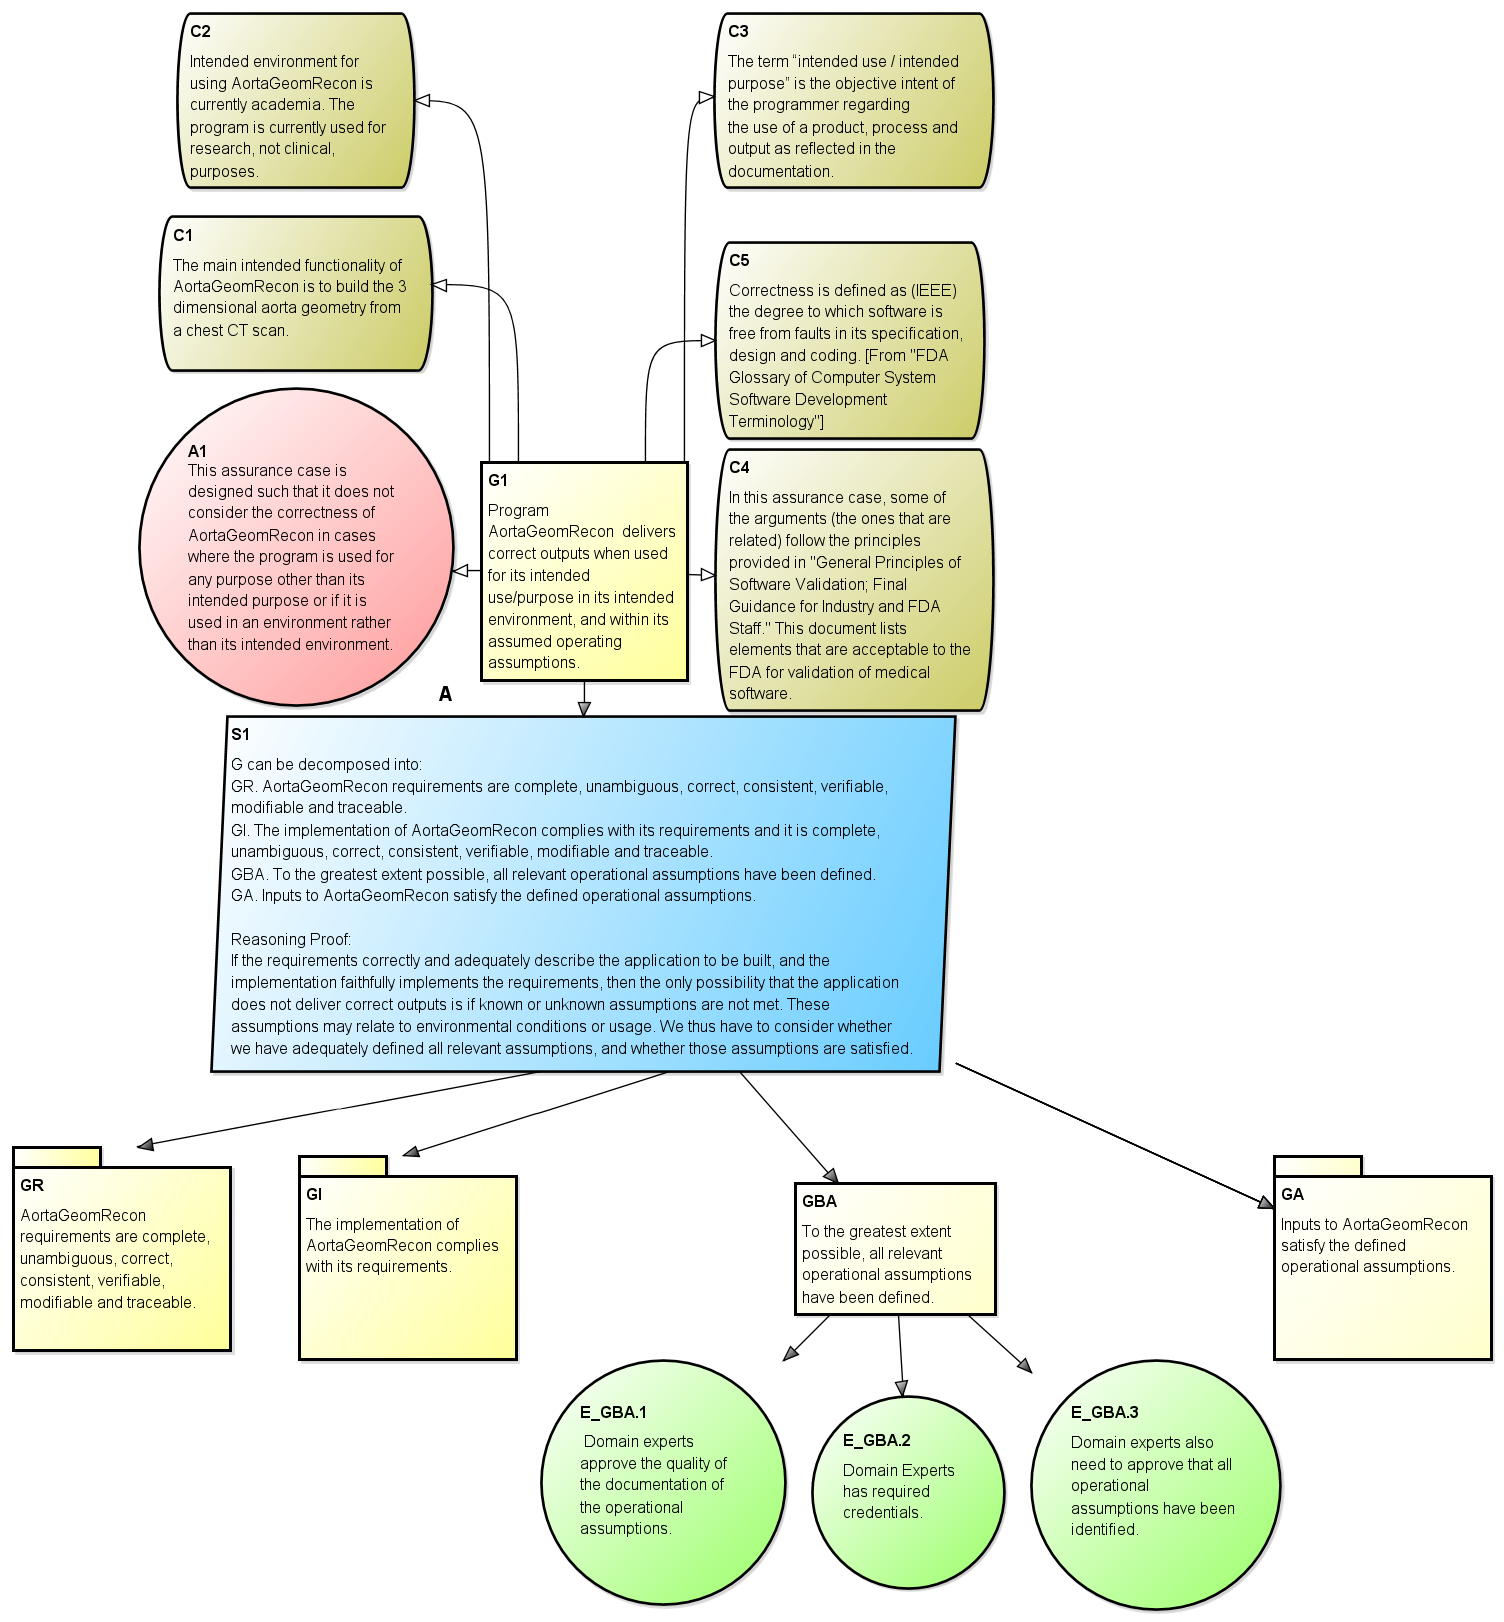
\includegraphics[width=0.99\textwidth]{figures/AC/Top_Level.png}}
    \caption[AGR Assurance Cases Top Level]{AGR Assurance Cases Top Level}
    \label{fig_agr_ac_top}
\end{figure}


\section{Assurance Case for Software Specification Requirements}

The first goal of getting a trusted software is having a complete, unambiguous, correct, consistent, verifiable, modifiable and traceable SRS that shows the complete breakdown of the requirements with mathematical notation, data models and instance models. The SRS is the foundation of the software development, and the design and the implementation will be based on the requirement document.

The Figure~\ref{fig_agr_ac_gr} demonstrates the claims on the goal of correct requirements of AGR. On the left branch, GR\_3C implies the goal of a complete, correct, and consistent documentation. Under this claim, the goal is separated based on each characteristic, and the corresponding evidence is presented as the leaf node. The S\_Correctness and S\_Completeness.4 node require a domain expert to review the quality of the document to ensure the documentation met the goal of the claims. The other characteristics of the documentation are supported with evidence as shown in the other branches in GR.

\begin{figure}[hp]
    \centering
    \fbox{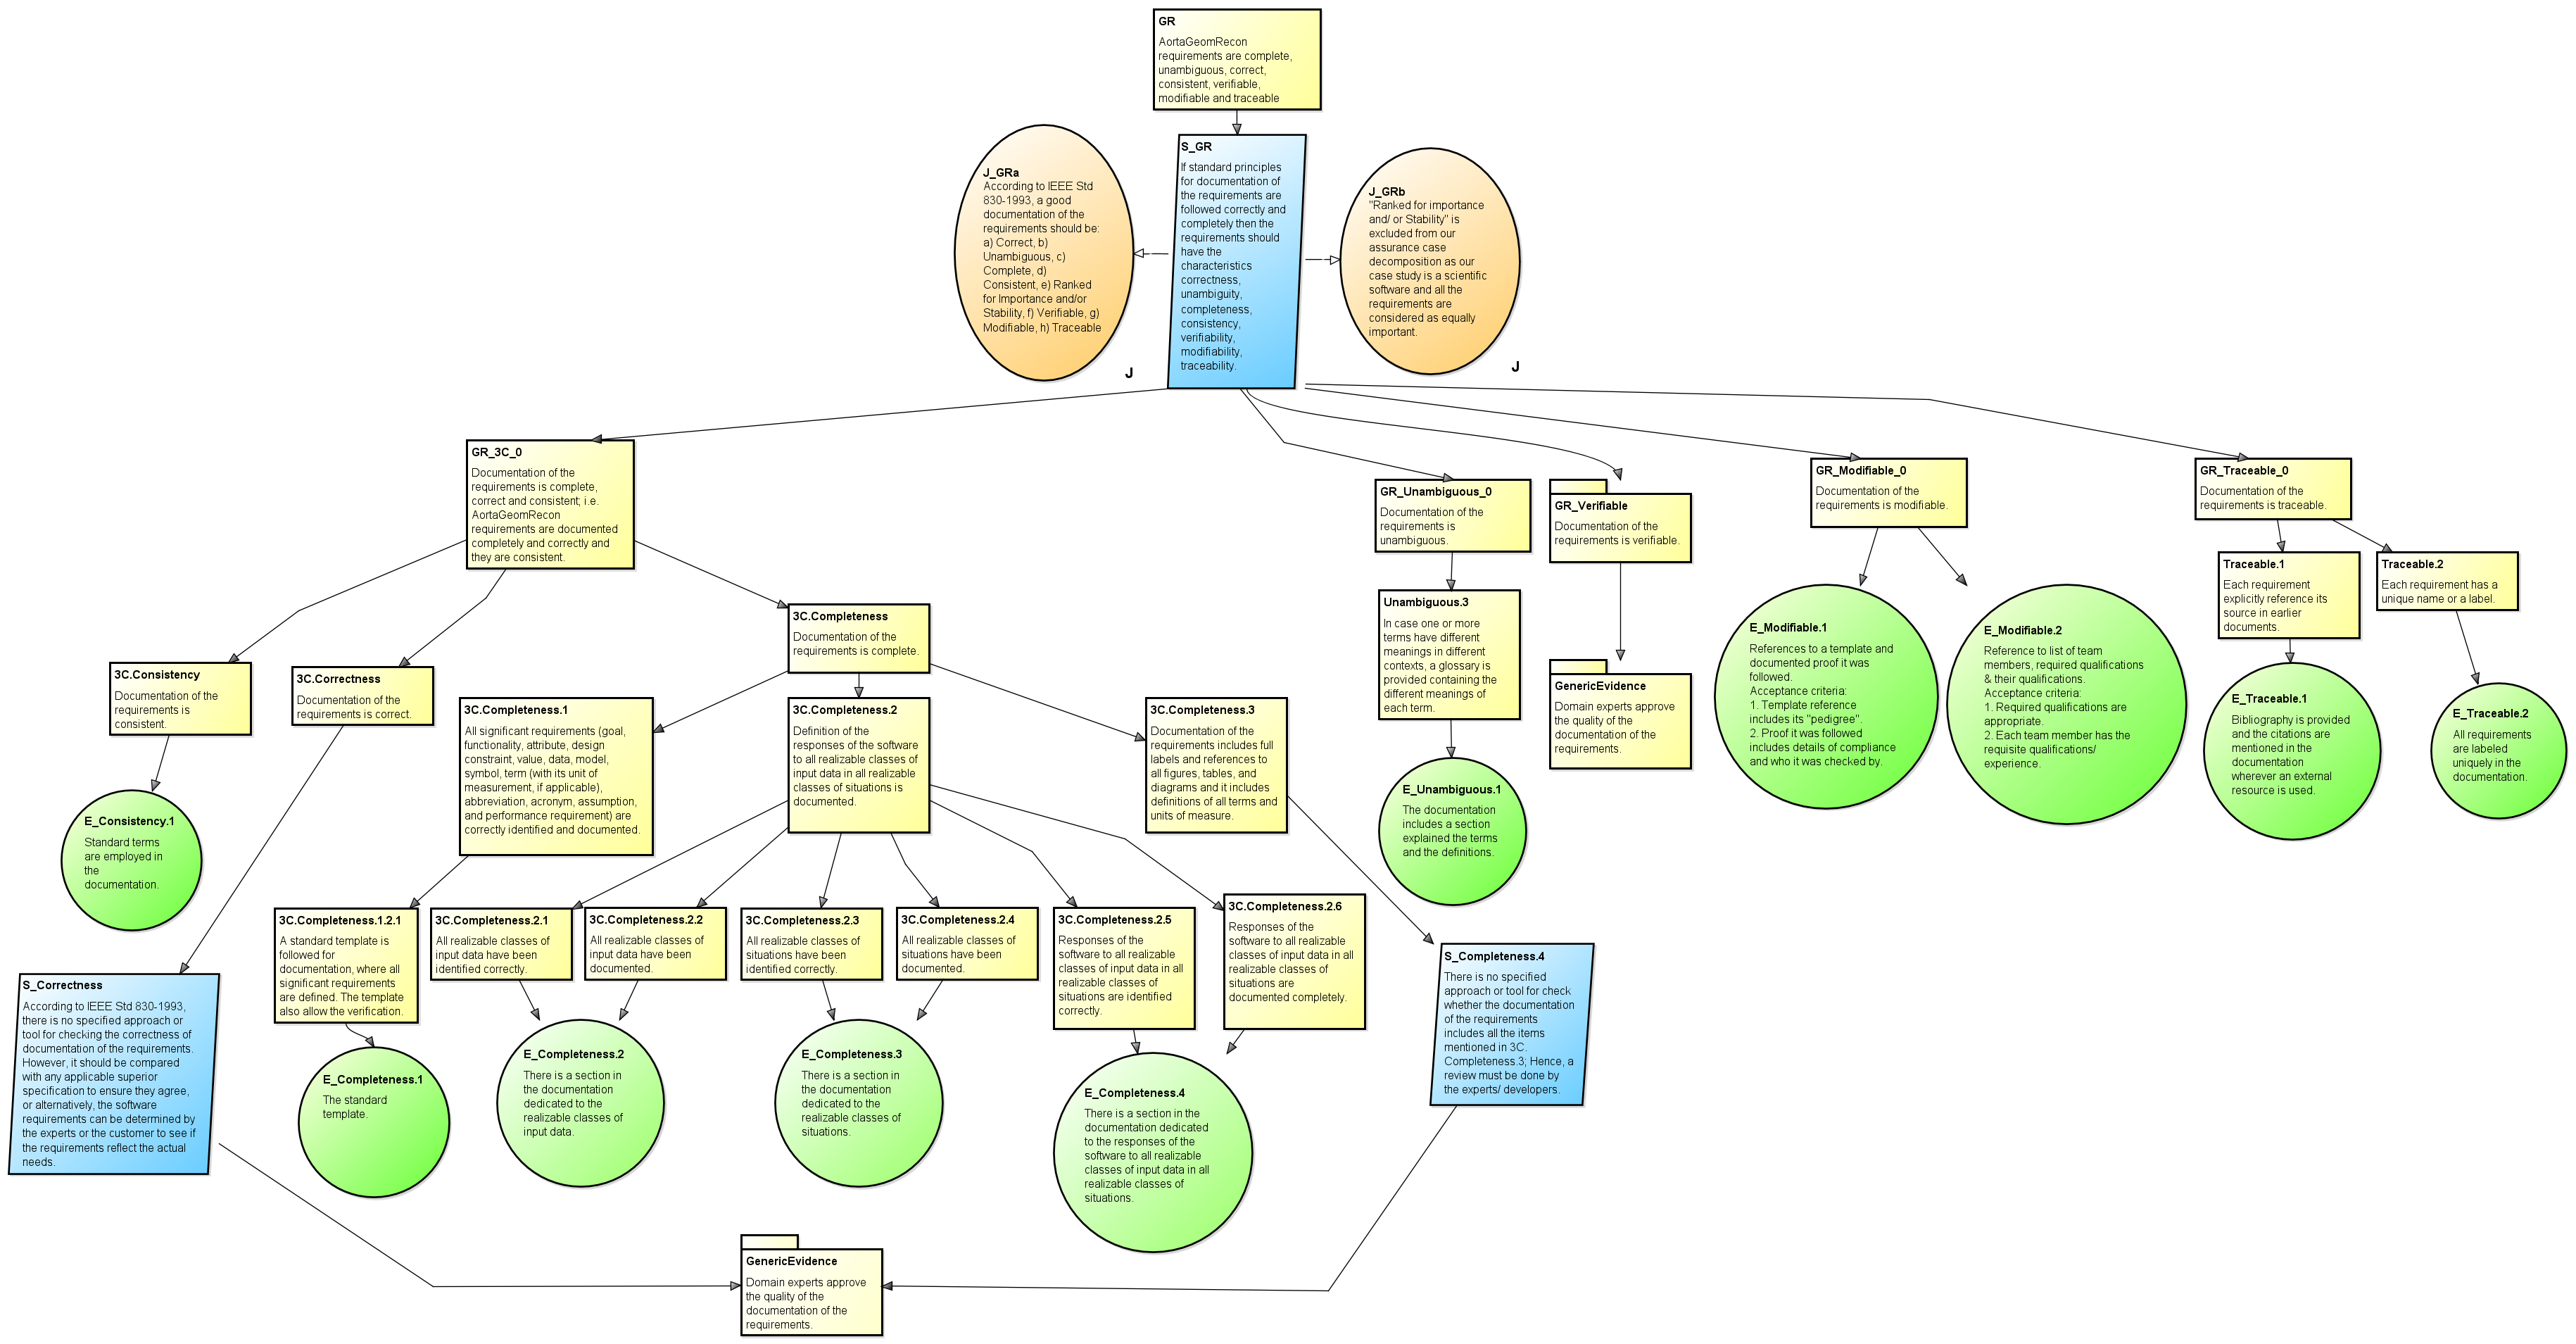
\includegraphics[width=1.3\linewidth, angle=90]{figures/AC/SRS/GSN_GR.png}}
    \caption[AGR Assurance Cases GR]{AGR Assurance Cases GR}
    \label{fig_agr_ac_gr}
\end{figure}

As explains in the assurance case GR, one of  most important statement of SRS having these characteristics is using a standard template. This document is attached as Appendix \ref{SRS}. Using  a standard template means that all necessary requirements have been defined, and it allows a domain expert who has used this template to verify the quality of the document. I used a template tailored for research software \cite{Smith2006}, which is the standard template in the evidence E\_Completeness.1, and all other evidences where a template is included.

\subsection{The Chapters of SRS}
The chapters in the SRS and some of the most important sections in the chapter are explained below:
\begin{itemize}
\item Reference Material

In this section, a Table of Symbols and an Abbreviations and Acronyms table are used to explain every symbol and Abbreviations used in the SRS document. These tables ensure the consistency and the unambiguous characteristics of the document, as the evidences E\_Consistency.1 and E\_Unambiguous.1 shown in the Figure~\ref{fig_agr_ac_gr}. They are located at the very beginning of the document, so the reader can first look at these tables before reading the entire document. 

\item Introduction

In the introduction section, I introduced the problems and the scope of the document.  These are subsections for explaining the purpose of document, abstracting the scope of requirements and defining the characteristics of the intended reader. This is provided for the reader to eliminates unambiguous in reading the document.

\item General System Description

The general system description includes a system context diagram which explains the relationship between the users, the inputs given by the user and the outputs of the AGR program. User responsibility and AGR responsibility are defined.

\item Specific System Description

In this section, I present more details about the problem and the specific system to solve the problem. The first subsection, Problem Description, discusses the definition of Organ Segmentation, the Coordinate Systems used in medical image problem, and Goal Statements. The goal for AGR is to extract the three-dimensional segmentation of the aorta.

In the next subsection, Solution Characteristics Specification, I started with the assumptions, as shown in Figure\ref{fig_agr_srs_a},  to clearly define the scope of the requirement document, as shown in Figure~\ref{fig_agr_srs_a}. In the subsection Data Definitions, I defined Voxel, Image/Slice, and Volume with mathematical notation so that the developer can easily interpret,  as shown in Figure~\ref{fig_agr_dd}. Next, in the subsection Instance Model, I showed the mathematical meaning of Region of Interest in Figure~\ref{fig_agr_im1}, and Segmentation in Figure~\ref{fig_agr_im2}, which are the two essential models that the developer must know to develop the solution. The Data Definitions and Instance Model sections are the evidences E\_Completeness.2, E\_Completeness.3 and E\_Completeness.4, which states that there is a section in the documentation dedicated to the realizable classes of input data, realizable classes of situation and the responss of the software to all realizable classes of input data in all realizable classes of situation. The Data Definition section defines the realizable classes of input data, the Instance Model section defines the realizable classes of situation and the response of the software.

\begin{figure}[H]
    \centering
    \fbox{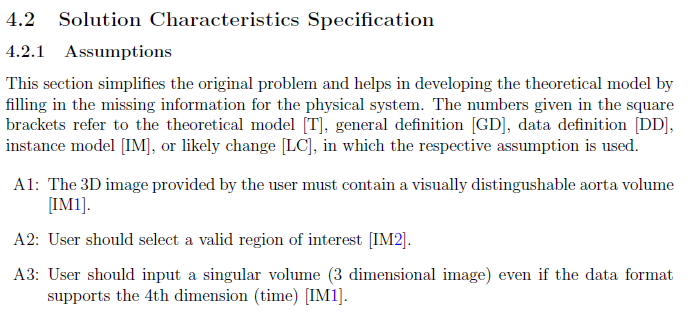
\includegraphics[width=\textwidth]{figures/AC/SRS/Assumptions.png}}
    \caption[AGR SRS Assumptions]{AGR SRS Assumptions}
    \label{fig_agr_srs_a}
\end{figure}

\begin{figure}[H]
    \centering
    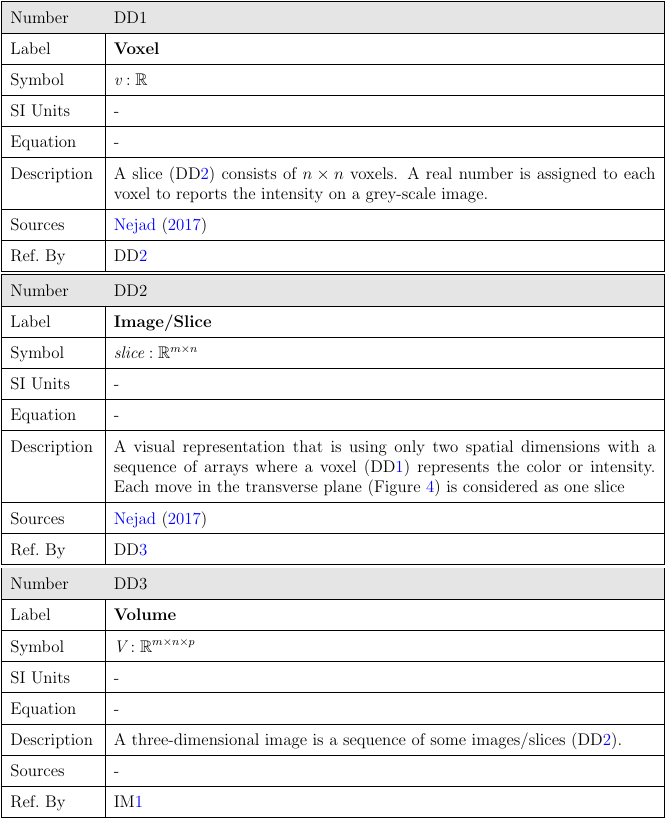
\includegraphics[width=\textwidth]{figures/AC/SRS/DD.png}
    \caption[AGR SRS Data Definitions]{AGR SRS Data Definitions}
    \label{fig_agr_dd}
\end{figure}

\begin{figure}[H]
    \centering
    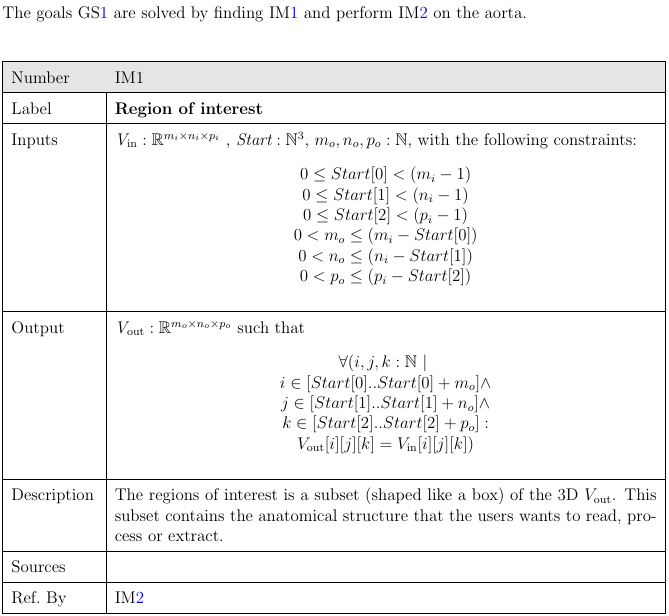
\includegraphics[width=\textwidth]{figures/AC/SRS/im1.png}
    \caption[AGR SRS Instance Model Region Of Interest]{AGR SRS Instance Model Region Of Interest}
    \label{fig_agr_im1}
\end{figure}

\begin{figure}[H]
    \centering
    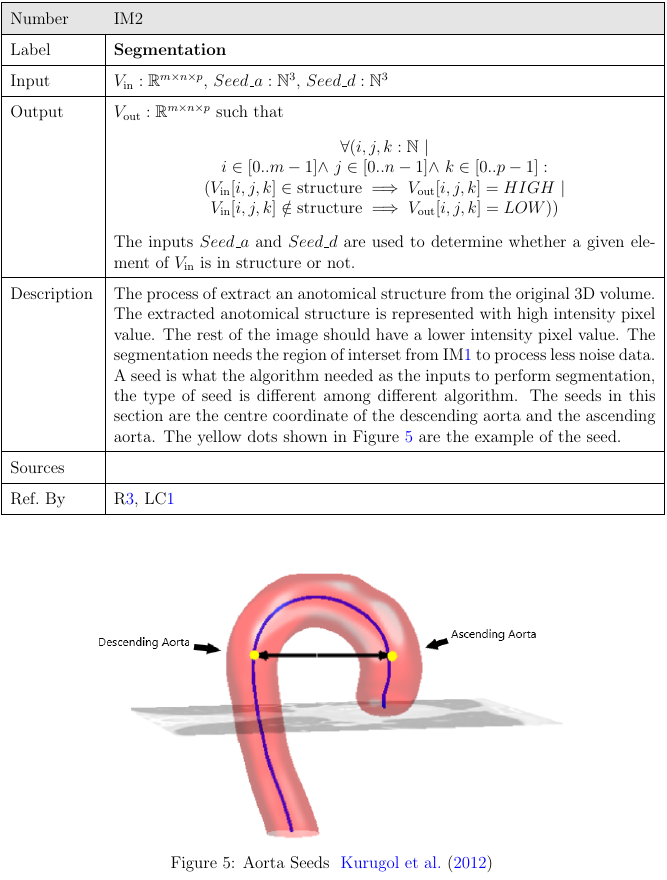
\includegraphics[width=\textwidth]{figures/AC/SRS/im2.png}
    \caption[AGR SRS Instance Model Region Of Interest]{AGR SRS Instance Model Region Of Interest}
    \label{fig_agr_im2}
\end{figure}


\item Requirements

With all the information in the document, I can now present the Functional Requirements and the Non-Functional Requirements for the program AGR. The Functional Requirements are defined by using the terms I presented in Data Definitions, Instance Model, and based on the other Functional Requirements, as shown in Figure~\ref{fig_agr_fr}. The Non-Functional Requirements usually have a measurement such as execution time, the effort of manual works. The Figure~\ref{fig_agr_nfr} demonstrates the Non-Functional Requirements, Usability, Safety, Learnability, Accurarcy and Consistency. The Functional Requirements and Non-Functional Requirements are labeled as the evidence  E\_Traceable.2 states.


\begin{figure}[H]
    \centering
    \fbox{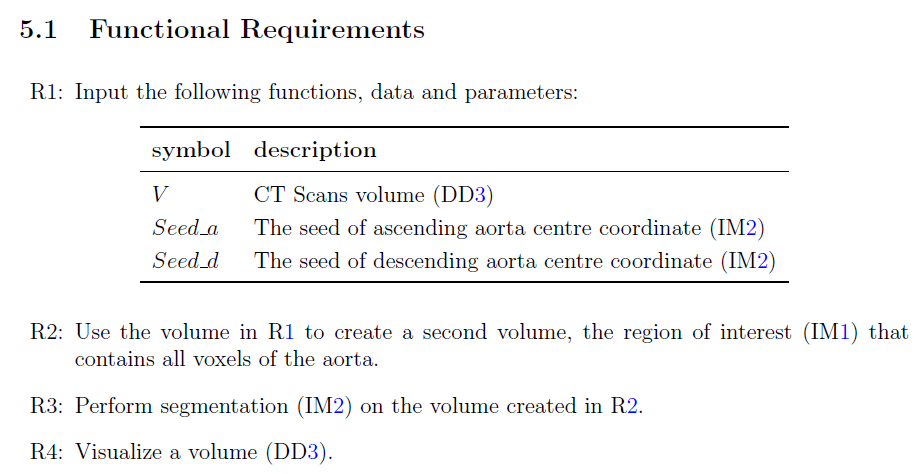
\includegraphics[width=0.75\textwidth]{figures/AC/SRS/Functional_Requirements.png}}
    \caption[AGR Functional Requirements]{AGR Functional Requirements}
    \label{fig_agr_fr}
\end{figure}

\begin{figure}[H]
    \centering
    \fbox{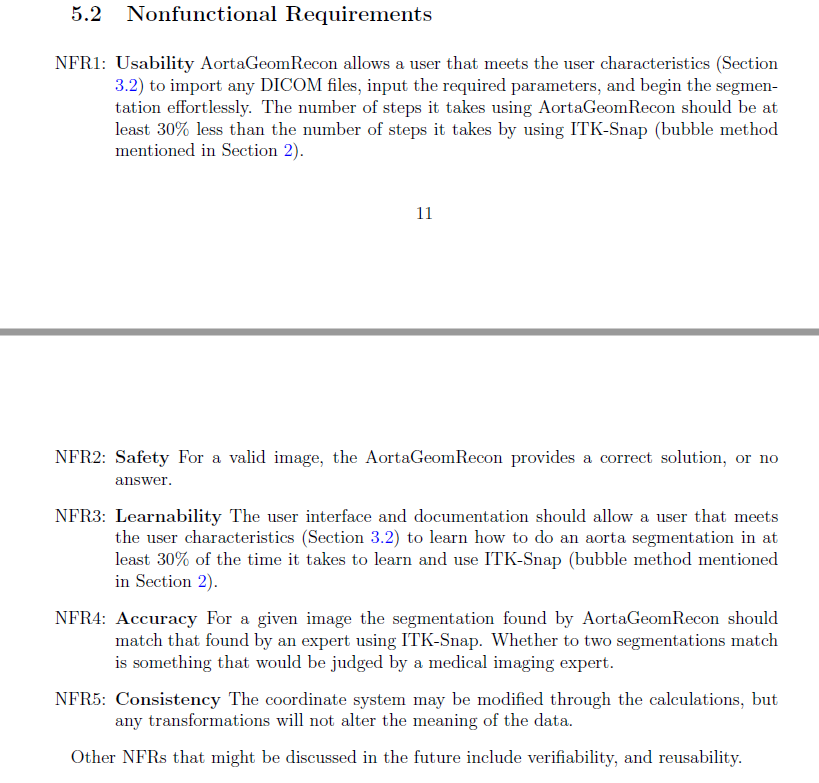
\includegraphics[width=0.75\textwidth]{figures/AC/SRS/NonFunctional_Requirements.png}}
    \caption[AGR Non- Functional Requirements]{AGR Non- Functional Requirements}
    \label{fig_agr_nfr}
\end{figure}

\item Likely Changes and Unlikely Changes

This section discussed the likely changes that the developer might expect a change in the future works, and the unlikely changes that is are not going to change for a justified reason. The only likely change discussed in the AGR's SRS is regarding the segmentation method. For different segmentation method, the inputs varies, since the segmentation method is a likely change, the inputs variables are also likely changes. The only unlikely change is the method of retrieving a region of interest. Most methods take a starting point and sizes in different dimensions to get the region of interest.

\item Traceability Matrix and Graphs

The traceability matrices are to provide easy references on what has to be additionally modified if a certain component is changed. Below shows the traceability matrices of different sections.
The Figure~\ref{fig_agr_tm_dd_im} is the traceability matrix of the Data Definitions and Instance Models. The Figure~\ref{fig_agr_tm_im_r} shows the relationship between the requirements and other sections. The Figure~\ref{fig_agr_tm_a} shows the relationship between the assumptions and other sections.
\begin{figure}[H]
    \centering
    \fbox{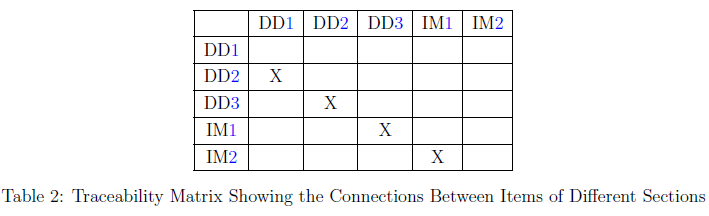
\includegraphics[width=0.7\textwidth]{figures/AC/SRS/tm_dd_im.png}}
    \caption[AGR Traceability Matrix between Data Definitions and Instance Model]{AGR Traceability Matrix between Data Definitions and Instance Model}
    \label{fig_agr_tm_dd_im}
\end{figure}

\begin{figure}[H]
    \centering
    \fbox{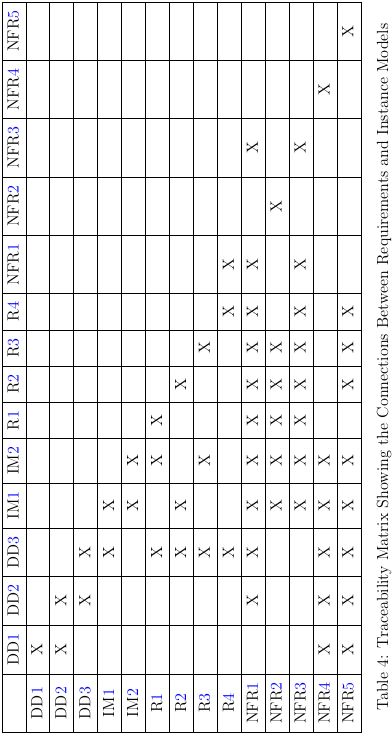
\includegraphics[width=0.8\textwidth]{figures/AC/SRS/tm_im_r.png}}
    \caption[AGR Traceability Matrix Between Requirements and Other sections]{AGR Traceability Matrix Between Requirements and Other sections}
    \label{fig_agr_tm_im_r}
\end{figure}

\begin{figure}[H]
    \centering
    \fbox{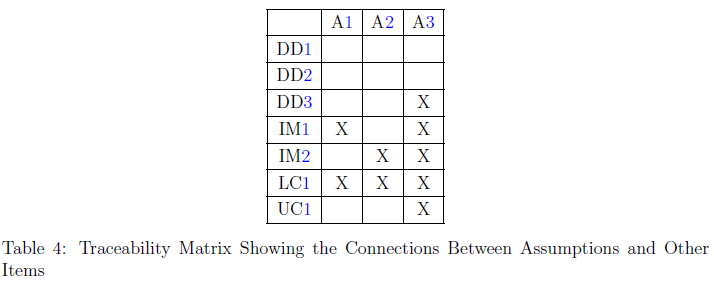
\includegraphics[width=0.8\textwidth]{figures/AC/SRS/tm_a.png}}
    \caption[AGR Traceability Matrix Between Assumptions and Other sections]{AGR Traceability Matrix Between Assumptions and Other sections}
    \label{fig_agr_tm_a}
\end{figure}

\item Bibliography
A Bibliography is provided at the end of SRS documentation, where it points to the template \cite{Smith2006} that I use to write this documentation, and a list of citations whenever an external resource is used. This is related to the evidences E\_Traceable.1, which states that a Bibliography is provided to include the citations of the external resource. The template is also related to E\_Modifiable.1, which states that the documentation references to a template and documented proof it was followed.

\end{itemize}

\subsection{Documentation Review}

Documentation Review is necessary to ensure the documentation's correctness and completeness. When there is an update in the documentation, I used GitHub Issues and post a documentation review request as shown in Figure~\ref{fig_agr_doc_review} to Dr. Spencer Smith, who has the requisite qualifications/experience to review the completeness and the correctness of the documentation. Additionally, the goal of the documentation being verifiable is also reviewed by Dr. Spencer Smith, and he approves the qualify of the documentation with the characteristic.

\begin{figure}[H]
    \centering
    \fbox{
\includegraphics[width=\textwidth]{figures/AC/SRS/Git_issues.png}}
    \caption[GitHub Repo Documentation Review Requests]{GitHub Repo Documentation Review Requests}
    \label{fig_agr_doc_review}
\end{figure}


\section{Assurance Case for the Implementation}
The goal of implementation is that it fully complies with the SRS. As Figure~\ref{fig_agr_ac_gi} shows, I argue this in two ways:

\begin{enumerate}
  \item I argue that the implementation of the requirements has been verified.
  \item I argue the design matches the requirement and that the implementation implies with the design, which implies that the implementation together matches the requirement.
\end{enumerate}

\begin{figure}[hp]
    \centering
    \fbox{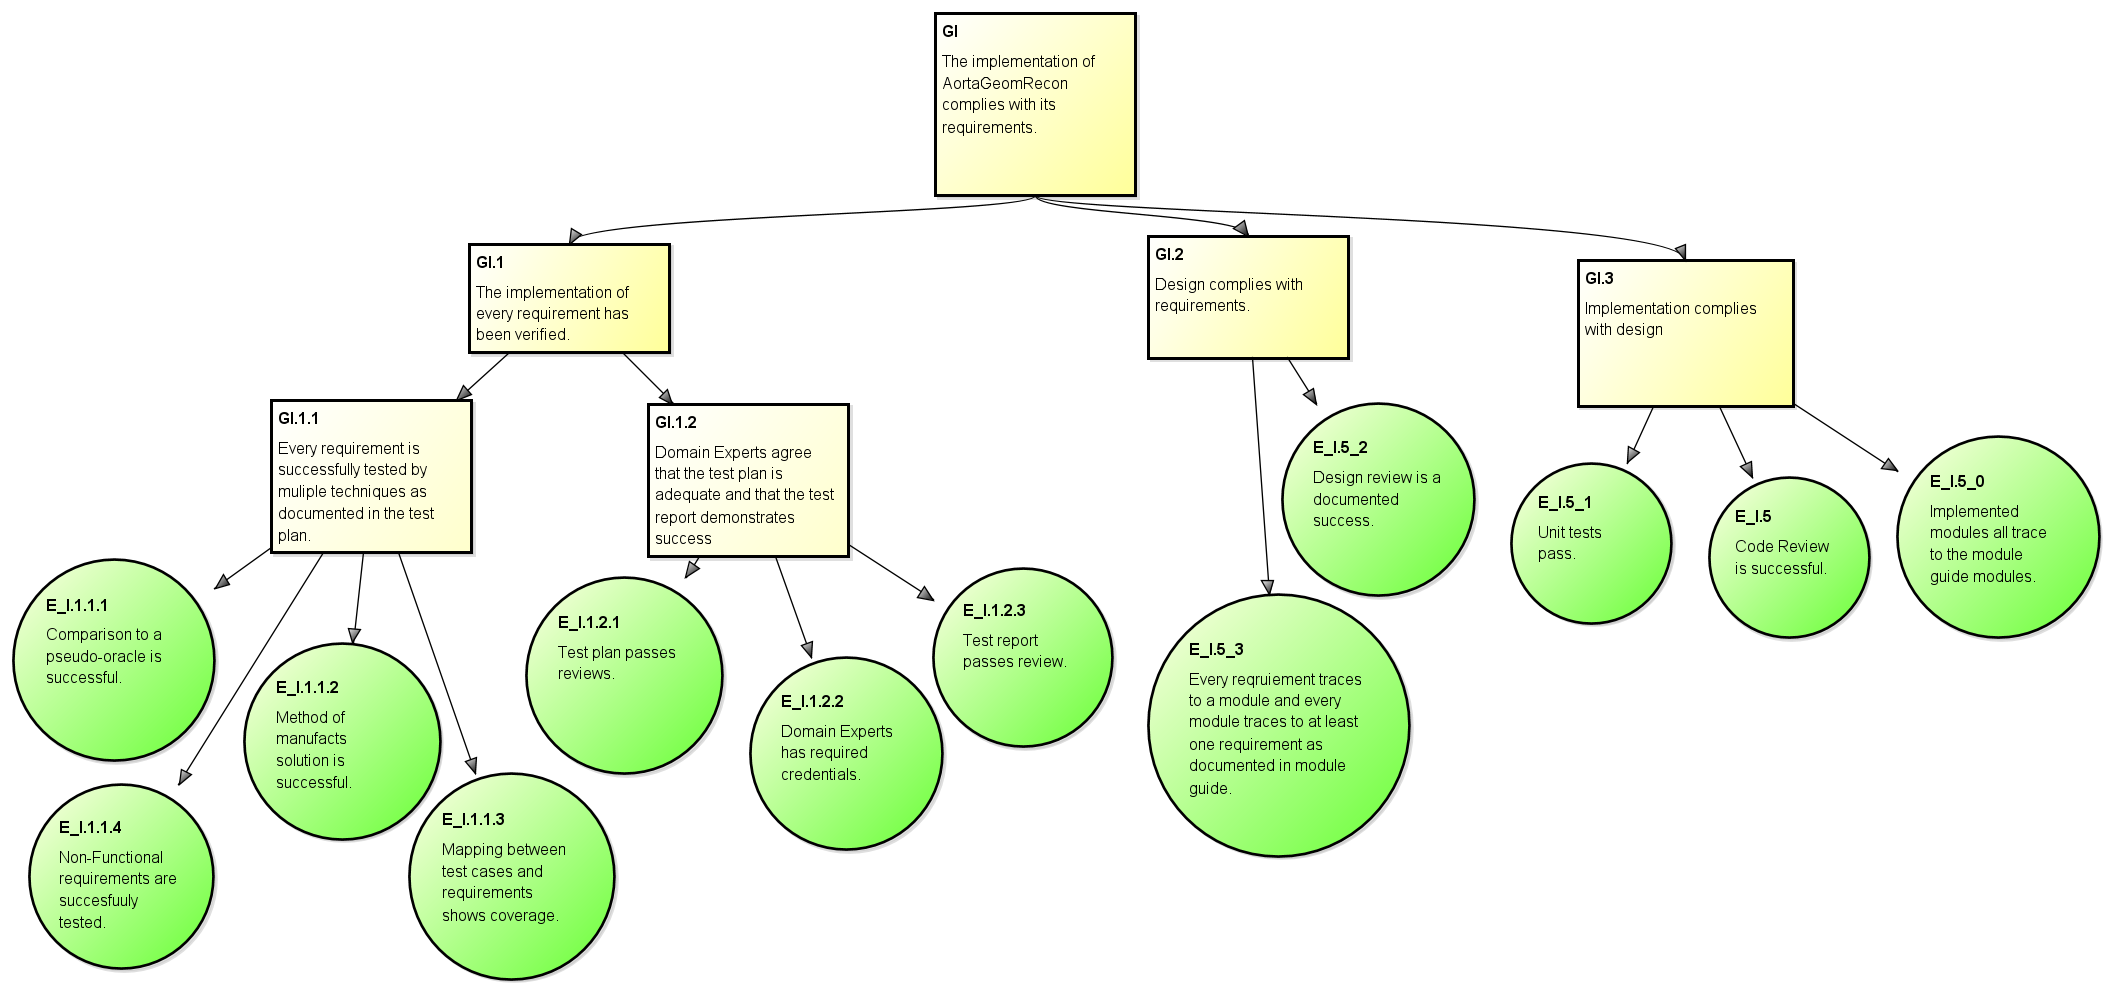
\includegraphics[width=1.3\linewidth, angle=90]{figures/AC/GI/GSN_GI.png}}
    \caption[AGR Assurance Cases For Implementation]{AGR Assurance Cases For Implementation}
    \label{fig_agr_ac_gi}
\end{figure}

In this section, I will focus on matching the developed artifacts to the evidence shown in Figure~\ref{fig_agr_ac_gi}. In the first sub-section I will discuss the test plan of the AGR, particularly on how I build the continuous integration test infrastructure, test cases and provide a test procedure to test all requirements of the software. Next, I will show my design documents, including the Module Guide to demonstrate system architecture, and a design document for detailed design explanation. Finally, I will talk about the Code Walkthrough and the Algorithm Review, which helped us to eliminates bugs, errors, and increase our confidence in the implementation's completeness, and correctness.

\subsection{Test Plan}

GI.1 states the goal of the implementaion of every requirement has been verified, so I need a test plan that is approved by a Domain Expert who has required credentials,  and the tests cases covers all of the Functional Requirement and Non-Functional Requirements. Unlike the other algorithm that can easily be tested with a ground truth test case, our ground truth case is build by using another more accurate method such as ITK-Snap's bubble method, then manually crosing the unwanted pixels.

In this section, I will discuss on how I build a ``Ground Truth'' data with a verified version of the algorithm, then compare it with the result generated from the new updated version of the algorithm using Dice Similarity. Next, I will show how I use GitHub Actions workflow as the continuous integration infruscturue perform static code analysis and continuous integration tests. Then, I provide a test procedure to cover the Functional Requirements and Non-Functional Requirements, as the evidences under GI.1 state in Figure~\ref{fig_agr_ac_gi}. Finally, I discuss on the test plan approval and the test report to includes the artifacts related to the evidences under GI.1.2.

\subsubsection{Build ``Ground Truth'' data}
Since learning on how to build a true ``Ground Truth'' test case by  using ITK-Snap is out of the scope of our project, I continuously build the ``Ground Truth'' test case with a previously verified version of the algorithm and a set of tuned hyperparameters. The only method to know which test case would be better is to have a manual review on  the generated  test case by a domain expert. The process of building the test case data is descibed as follow:

\begin{enumerate}
  \item Generate a test case data with the previous satisfied version of the algorithm.
  \item Generate a test case data with the new version of the algorithm.
  \item Calculate the Dice similarity coefficient (DSC) of the two test case data.
  \item If there is a strong difference in the DSC value, use visualization tool such as 3D Slicer to see the actual difference, and decide which test case to keep for the future.
\end{enumerate}

The Dice similarity coefficient (DSC) was used as a statistical validation metric to evaluate the performance of both the reproducibility of manual segmentations and the spatial overlap accuracy of automated probabilistic fractional segmentation of MR images \cite{ZOU2004178}. With a small DSC value, the evidence E\_1.1.1 is achieved by comparing a new generated result with a pseudo-oracle. The statement of the evidence E\_1.1.2 is also correct, which implied that a chosen approach or methodology has led to the creation of software that functions as intended, meets user requirements, and adheres to quality standards.

\subsubsection{GitHub Actions workflows}
This leads to our Continuous Integration infrastructure, implemented with GitHub Actions workflow. A workflow is a configurable and automated process that will run one or more jobs on the desired system. GitHub Actions workflow used a YAML file to define the events and the commands to be executed on the temporary system, which has the build of the repository \cite{GitHubActions}.

I have set up two automated process which happens on each ``push" event and ``pull" event. A ``push" event implies that something is changed in one or multiple commits, therefore there is a need to verify whether the commits have bugs that need extra fixes. A "pull" event happens when a feature branch is going to merge with the main branch. Since our main branch is protected, any update to the main branch must be merged by using a pull-request. Before a pull-request can be approved, the continuous integration tests are examined and until there are no errors, a pull-request cannot be merged with the main branch. 

The first automated process is a linter. A linter is a tool for static code analysis to flag programming errors, bugs, stylistic errors and suspicious constructs. I used Python Flake8 as our linter to find bugs and errors, and ensures that program's readability by striking the source code with Google's published  Python Style Guide. \cite{Linter}

The second automated process is our continuous integration tests. By setting up Git Large File System (LFS) and upload to pre-build ground truth test data in the repository, I can now pass the cropped volume as the input data, the same aorta seeds and the hyperparameters that I have used to generate the ground truth test data to the algorithm and verify the results. By calculating the DSC value of both images, I can now set a limit such that the update to the algorithm is passing or failing our test if  the DSC value is within the limit. This indicates that our evidence E\_I.5\_1 is accomplished.

\subsubsection{Test Procedure}

In this section, I will introduce our test procedure for Functional Requirements and Non-Functional Requirements.

The Functional Requirements can be tested by generating a segmentation result from scratch in 3D Slicer. Without loading a MRMLscene file on purpose, 3D Slicer is in its default state. The test procedure for testing the Functional Requirements is described as follow:

\begin{enumerate}
  \item Open 3D Slicer.
  \item Load a DICOM file using 3D Slicer's DICOM database.  
  \item Generate a ROI object using 3D Slicer's Volume Rendering module, as described in user manual.
  \item Generate a cropped volume using 3D Slicer's Crop Volume module, as described in user manual.
  \item Load \progname{}DisplayModule, click on the ``Apply" button to proceed to next step.
  \item Input the aorta seeds.
  \item Input the hyperparameters.
  \item Click on the ``Apply" button.
  \item Visualize the segmentation result.
\end{enumerate}

If step 1-4 did not proceed correctly, there is an error with 3D Slicer, which is out of the scope of the project. If an error happens in step 5-7, there might be an error with the plugin as a scripted module. Otherwise, step 8 generates a result is only concerns with the hyperparameters and the algorithm's implementation, and step 9 is affected by 3D Slicer and the result generated from step 8. This test procedure has all Functional Requirements match to a step, where R1 matches to step 2, R2 matches to step 3, R3 matches to step 8, and R4 matches to step 9. Thus, I have our evidence E\_1.1.3.

The Non-Functional Requirements is difficult to test, because each user with different experience could result in different learning time, and total time it takes from scratch to generating a segmentation result. The test procedure used in Functional Requirement test can be used for Non-Functional Requirements test. Both NFR1 Usability and NFR3 Learability requires a measurement in time comparing to another software. NFR2 Safety, NFR4 Accuracy, and NFR5 Consitency requires a verification in the segmentation result. NFR4 Accuracy also requires a segmentation result generated by ITK-Snap. By performing all of the above action, I have all Non-Functional Requirements tested, which is the evidence E\_1.1.4.

\subsubsection{Test Plan Approval and Test Report}
GI.1.2 states that a domain expert with required credentials must review the test plan, and the test report. The test plan is reviewed by Dr. Spencer Smith, and our test report is partially automatically generated by GitHub Actions workflows, as shown in the Figure~\ref{fig_agr_test_report}.

\begin{figure}[H]
    \centering
    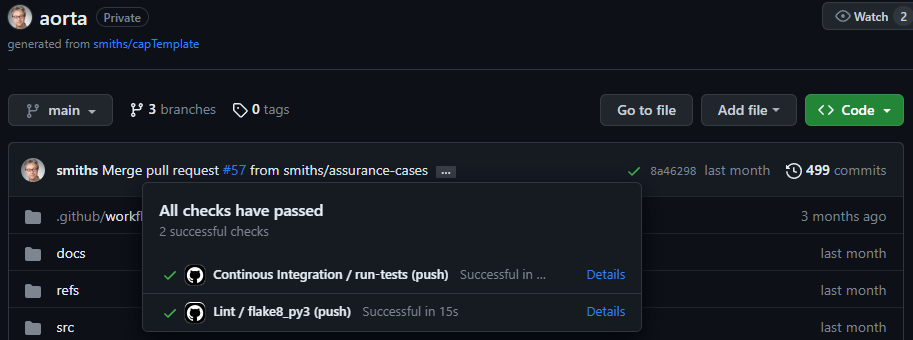
\includegraphics[width=0.9\textwidth]{figures/AC/GI/test_report.png}
    \caption[AGR Test Report]{AGR Test Report}
    \label{fig_agr_test_report}
\end{figure}

The GitHub will send an email to all the contributors when some checks were not successful, thus I are awared of these errors.

\section{The Design Documentation of the \progname{}}

In this section, we will discuss the design documents of the \progname{}. There are multiple aspects of the design document to discuss:

\begin{enumerate}
\item System architecture, or high levels design.
\item Detailed design explaning how the algorithm works.
\end{enumerate}

The first item is presented with a Module Guide, and the second item is presented with a source code documentation generator, which generates the binary in HTML and is hosted on a web server.

\subsection{Module Guide}

An important document to show that the design is complete, correct, and consistent design is Module Guide (MG), which  is attached as Appendix \ref{MG}. As explained previously, MG demonstrates the system architecture, or the high level design of the \progname{}. The designer typically keeps these anticipated changes isolated to a single module so if the change happens, only one module is impacted. The anticipated changes are listed in the Figure~\ref{fig_agr_ac} below.

\begin{figure}[H]
    \centering
    \fbox{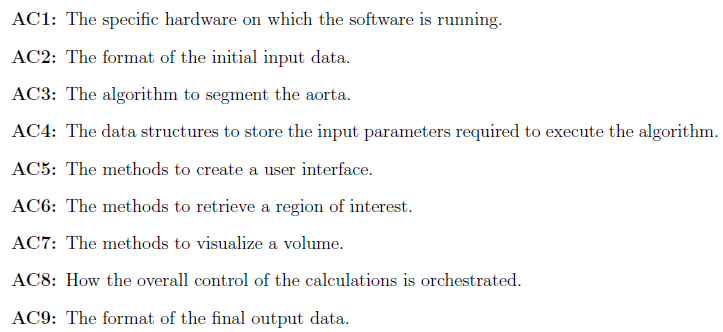
\includegraphics[width=\textwidth]{figures/AC/MG/Anticipated_Changes.png}}
    \caption[AGR Anticipated Changes]{AGR Anticipated Changes}
    \label{fig_agr_ac}
\end{figure}

Modules are decomposed according to the principle of “information hiding” proposed by Parnas et al. (1984). The Secrets' field in a module decomposition is a brief statement of the design decision hidden by the module. The Services' field specifies what the module will do without documenting how to do it. The module hierarchy and a part of the module decomposition is demonstrated in Figure~\ref{fig_agr_modules} and Figure~\ref{fig_agr_md}. For each module, a suggestion for the implementing software is given under the Implemented By title. If the entry is OS, this means that the module is provided by the operating system or by standard programming language libraries. AGR means the module will be implemented by the AGR software.

\begin{figure}[H]
    \centering
    \fbox{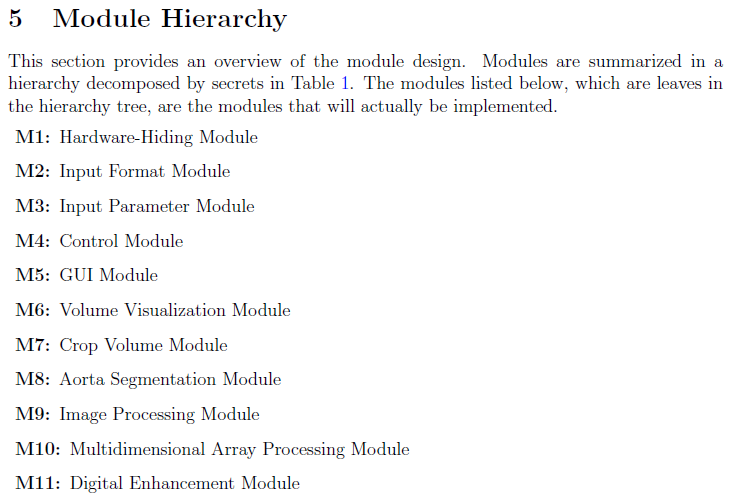
\includegraphics[width=\textwidth]{figures/AC/MG/Modules.png}}
    \caption[AGR Modules]{AGR Modules}
    \label{fig_agr_modules}
\end{figure}

\begin{figure}[H]
    \centering
    \fbox{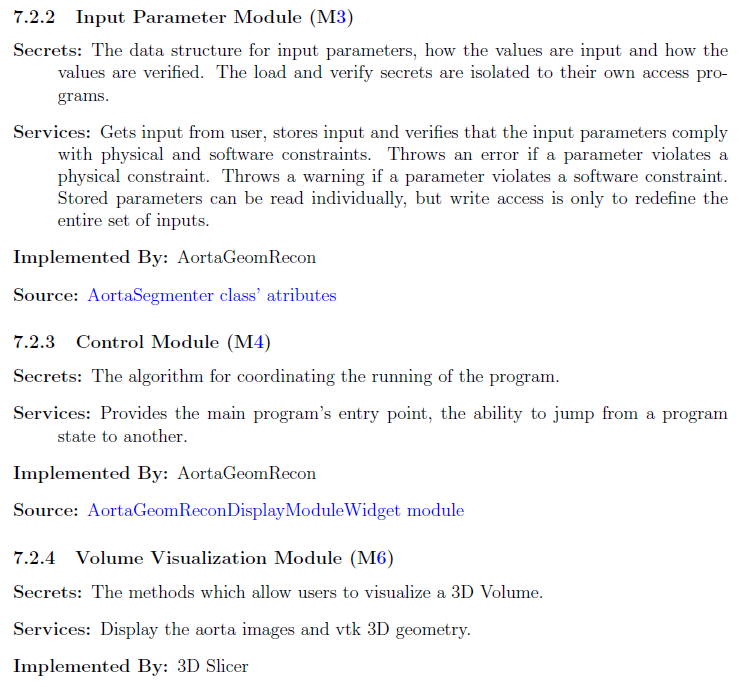
\includegraphics[width=\textwidth]{figures/AC/MG/Modules_Decomposition.png}}
    \caption[AGR Module Decomposition Example]{AGR Module Decomposition Example}
    \label{fig_agr_md}
\end{figure}

Now that I have listed the anticipated changes and the modules, I use traceability matrices to show the relationships between the modules and the anticipated changes, and between the modules and the requirements, as shown in Figure~\ref{fig_agr_mtm}. This indicates that the design is fully complying with the requirements, as I stated in the evidence E\_I.5\_3, under the GI.2 in the Figure~\ref{fig_agr_ac_gi}.

\begin{figure}[H]
    \centering
    \fbox{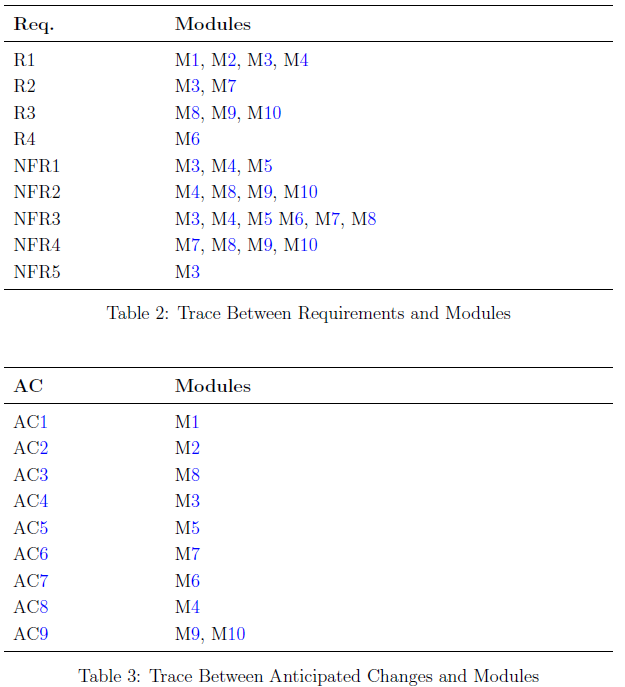
\includegraphics[width=0.7\textwidth]{figures/AC/MG/TM.png}}
    \caption[AGR Modules Traceability Matrices]{AGR Modules Traceability Matrices}
    \label{fig_agr_mtm}
\end{figure}

On top of relating the modules to the requirements, I am relating the actual source code to the modules, which is a strong evidence of our implementation complies with the requirements, as shown in Figure~\ref{fig_agr_mtm_modules_code}. Module 11 Digital Enhancement Module is an example of Module mapping to a piece of the source code. In the comments on top, I added the source file where this piece of the source code is located, as well as the exact places with GitHub and the exact lines highlighed. This table demonstrates that the implemented modules all traces to the module guide modules, as stated in the evidence E\_I.5\_0.

\begin{figure}[H]
    \centering
    \fbox{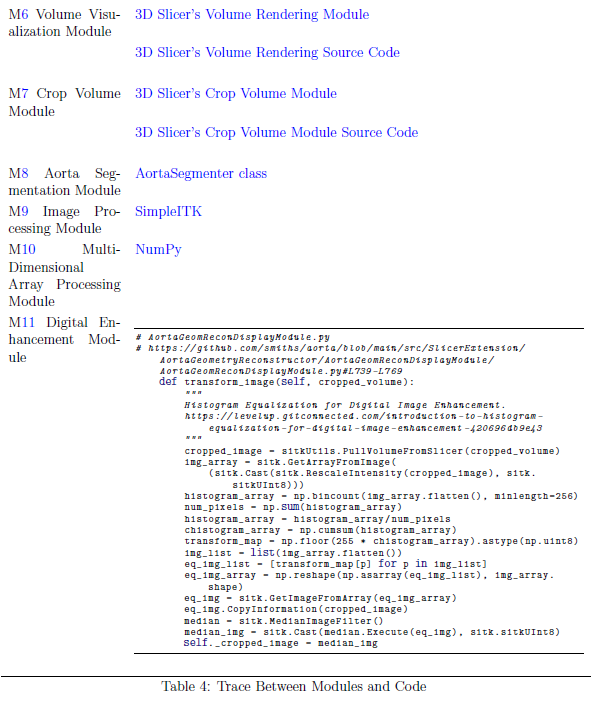
\includegraphics[width=0.9\textwidth]{figures/AC/MG/TM_modules_code.png}}
    \caption[AGR Part Of The Traceability Matrix On Modules And Code]{AGR Part Of The Traceability Matrix On Modules And Code}
    \label{fig_agr_mtm_modules_code}
\end{figure}

\subsection{Detailed Design Document}
The purpose of the Design Document \cite{DD} is to explain in details how the algorithm works, and why it worked. Similar to what section \ref{algo} wrote, the design document explains in plain text the workflow of the algorithm. The design document is a piece of evidences that demonstrate unambiguity. Moreover, this document can let the domain expert to do a design review  without reading the source codes directly,  which helps building the evidence E\_I.5\_2.

To show and automate the detailed design, I used Sphinx, a Python Documentation Generator that can build module's documentation from the comments in the source code. Moreover, using reStructuredText to write the Algorithm Overview, I can build HTML code which can be published on a web server, as shown in Figure~\ref{fig_agr_dd}, which shows the index page of the \href{https://joviel25.github.io/AortaGR-design-document/index.html}{website}. 

\begin{figure}[H]
    \centering
    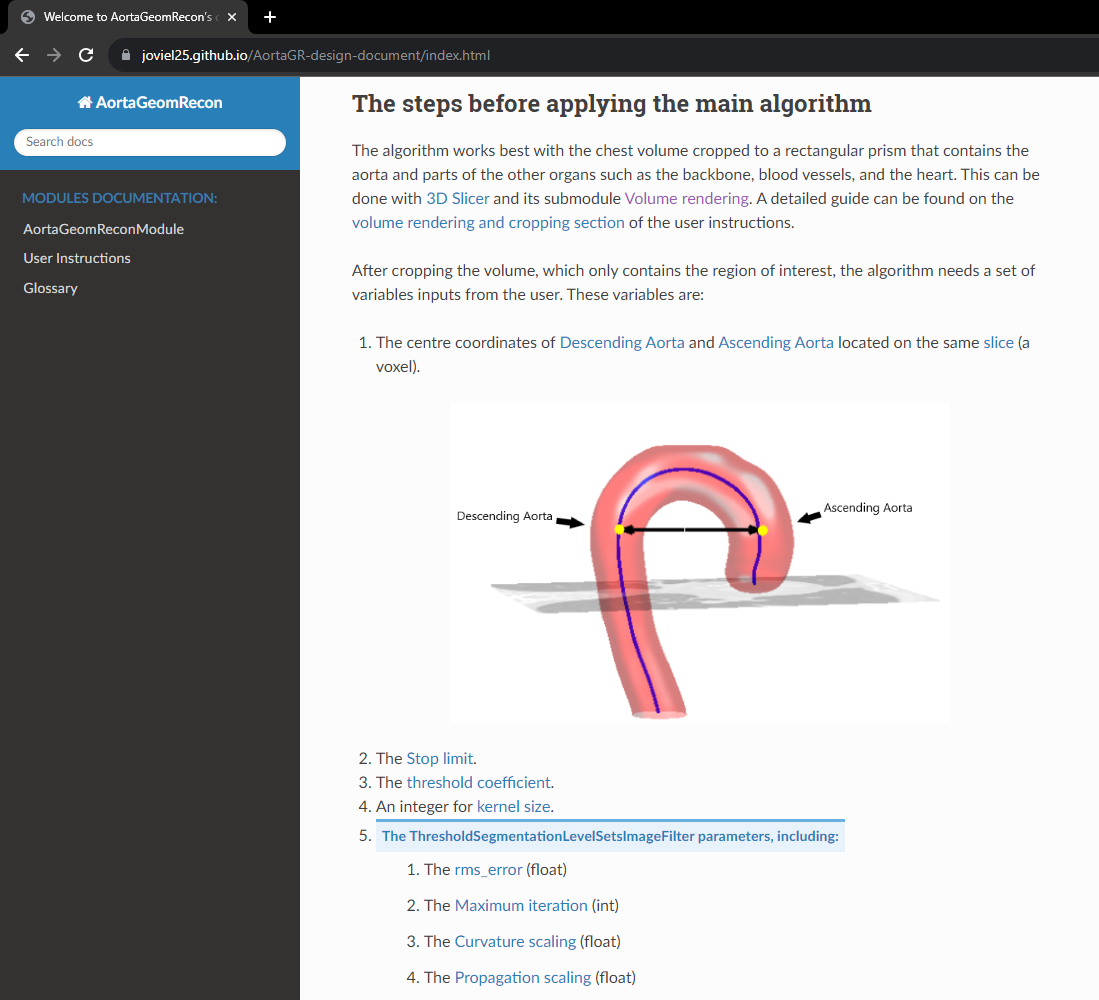
\includegraphics[width=0.65\textwidth]{figures/AC/DD/Main_page.png}
    \caption[AGR Design Document Website]{AGR Design Document Website}
    \label{fig_agr_dd}
\end{figure}

Another important section in detailed design document is the Glossary. It has a rich vocabulary explanation, images, and links to the outside source to let the reader understands as much as possible, as demonstrated in Figure~\ref{fig_agr_dd_glossary}.

\begin{figure}[H]
    \centering
    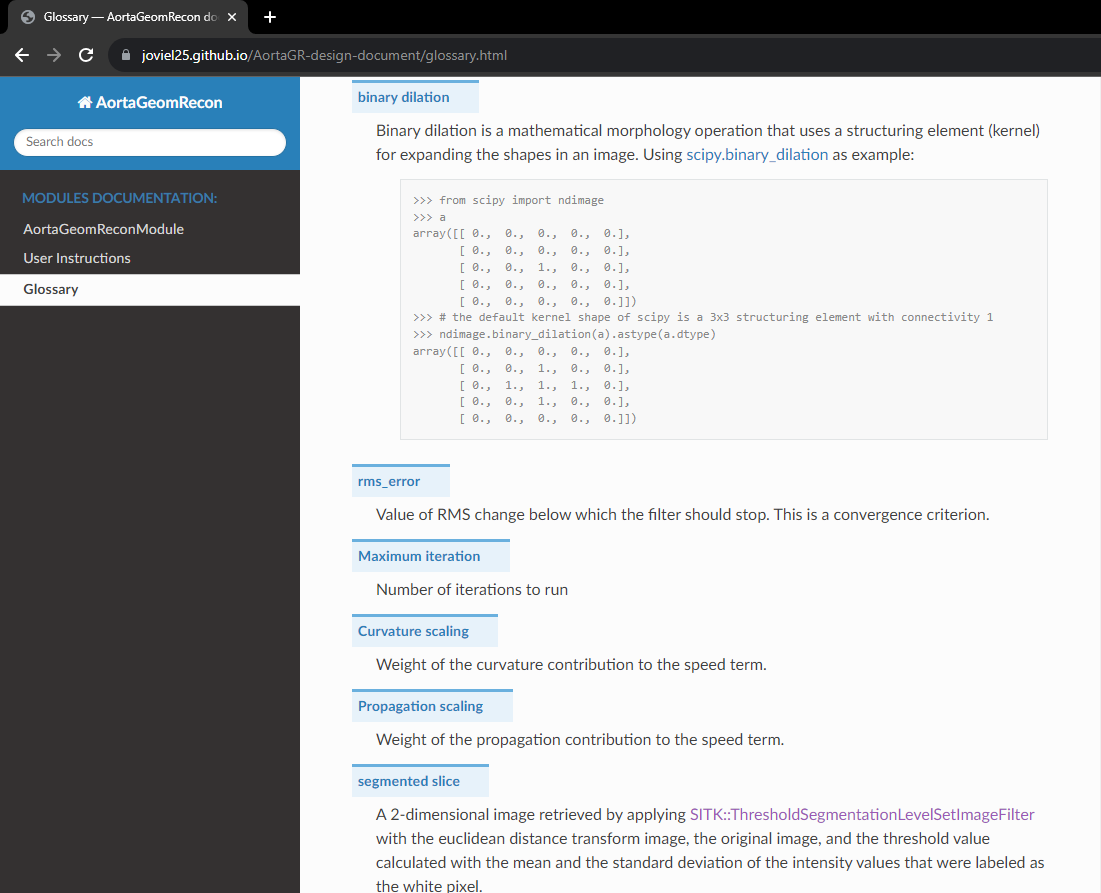
\includegraphics[width=\textwidth]{figures/AC/DD/Glossary.png}
    \caption[AGR Design Document Glossary]{AGR Design Document Glossary}
    \label{fig_agr_dd_glossary}
\end{figure}


\subsection{Algorithm Review}

The Algorithm Review started with a Code Walkthrough. A Code Walkthrough is a systematic and collaborative process in software development where a team of developers, designers, and stakeholders review and analyze a piece of code, typically with the aim of identifying defects, potential issues, and improvements \cite{Corporate_2023}. During a Code Walkthrough, participants examine the code line by line, discussing its design, functionality, readability, maintainability, and adherence to coding standards. The process involves both the author of the code and other team members, fostering knowledge sharing and collective learning. The goal is to catch issues and enhance the codebase through collective expertise.

We contrast a Code Review with an Algorithm Review. In an Algorithm Review, we present the algorithm to the domain expert and asking them if the detailed design fulfill the implementation objectives. In a Code Review, we are inspecting the implementation and verifying if the implementation has followed the design. 

In this section, I will discuss the Code Review with Kailin Chu, and the key takeaways from this meeting. Then, I will discuss the Algorithm Review with Dr\. Dean Inglis, which the meeting has reinforced our confidence in the design. Finally, I will briefly introduce the tools that we have used in both meetings.

\subsubsection{Code Review with Kailin Chu}
The Code Review was done with Kailin Chu, who is a biomedical engineering student and started working the semi-automacial aorta segmentation algorithm as a summer researcher. The meeting happened on Thursday, April 20, 2023, and the duration is about an hour. Along with Dr. Smith Spencer, I was aiming to increase our confidence in the code via a Code Walkthrough. This code walkthrough did not increase our confidence in the software and it became a Code Review, because the code was developed by Kailin from two years ago, so some details and design decisions were missing, and some variables were decided by trial and error. Despite that the code walkthrough has turned into an algorithm review, and it did not achieve what I wanted in the first place, this meeting was still very helpful. Originally, the old method to generate a label image that we have discussed in the section \ref{label_map} is partialy random when the algorithm is segmenting on the superior direction. This happened when from axial view going toward the head direction, we are observing that ascending aorta and the descending aorta is going to merge into one piece. However, the segmentation on the aortic arch requires the algorithm to generate a label image to cover part of the descending aorta. This coverage is sometime missing when executing on certain test case. Knowing that this part of the algorithm was partially based on trial and error, I was confident on improving the algorithm by using the idea of centroids. By using two centroids, one centroid on the ascending aorta and another on the descending aorta, the centroids can keep track of the most centered position of ascending aorta and descending aorta when the aortic arch region is reached. Thus, it generates a better label image, and it will generate a more accurate segmentation result.

\subsubsection{Algorithm Review with Dr. Dean Inglis}

The algorithm review was conducted with Dr. Dean Inglis, an experienced professor, Medical Image Analyst, and Software Developer. The meeting happened on May 17, 2023, and the duration is about one and half hour. I presented our segmentation algorithm to him and requested validation of our approach or suggestions for a potentially superior algorithm. Dr. Dean Inglis provided his insights on the algorithm, which I meticulously recorded on the GitHub issue tracker. These insights will guide the developer responsible for enhancing the program. This meeting significantly reinforced our confidence in both the software and our endeavors, because the methods discussed in the section \ref{label_map}, \ref{distance_map}, and \ref{methodologies}  were very common in image analysis. The level sets segmentation is also a often used technique for image segmentation. This indicates that the evidence E\_I.5 is accomplished.

\subsubsection{Tool used in Algorithm Review}

Spyder is a free and open source scientific environment written in Python, for Python, and designed by and for scientists, engineers and data analysts. The Variable Explorer allows the user to interactively browse the variables and the objects in debugging mode \cite{raybaut2009spyder}.
\begin{figure}[H]
    \centering
    \fbox{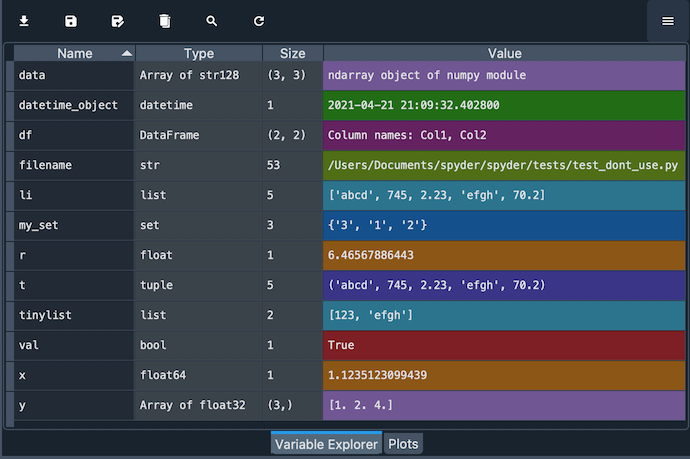
\includegraphics[width=0.8\textwidth]{figures/AC/AR/variable-explorer-standard.png}}
    \caption[Spyder Variable Explorer]{Spyder Variable Explorer \cite{raybaut2009spyder}}
    \label{fig_spyder_ve}
\end{figure}

This feature allows us to execute the program step by step, and see what happens to the variable (segmentation result) when executing the segmentation algorithm. 



\section{Assurance Case for Operational Assumptions}

\begin{figure}[H]
    \centering
    \fbox{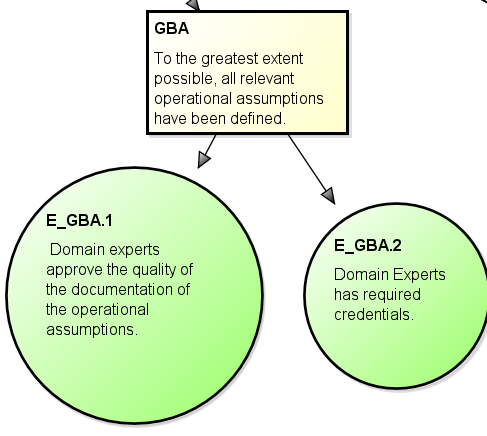
\includegraphics[width=0.5\textwidth]{figures/AC/GBA/GBA.png}}
    \caption[AGR Assurance Case Operational Assumptions]{AGR Assurance Case Operational Assumptions}
    \label{fig_agr_ac_gba}
\end{figure}

The evidence for the statement ``To the greatest extent possible, all relevant operational assumptions have been defined" is quite simple as all that is required is a qualified Domain experts approve the quality of the documentation. However, finalizing this evidence takes significant effort from the beginning of the project to the end of the project, because I want to continuously improve the quality of the content matching the most recent updates of the software.

In this section, we will present two methods to define all relevant operational assumptions. The first method is a User Manual, which is written in plain text and multiple screenshots. The second method is a User Instructional Video, which includes voice over to guide the user step by step.

\subsection{User Manual}
A user manual serves the purpose of documenting all operational assumptions. When the user gets unexpected results by using this software, they should be able to refer to the user manual to see what pieces are different. Our user manual is initially located in GitHub repo's README, as shown in Figure~\ref{fig_agr_git_um}, which is only available to the developers invited as the GitHub project contributors. The content includes the installation of the software, importing the extension modules, import inputs data, and perform segmentation. The user manual is also available publicly on the \href{https://joviel25.github.io/AortaGR-design-document/UserInstructions.html}{design document website}, assuming that the users might not be the repository contributors.

\begin{figure}[H]
    \centering
    \fbox{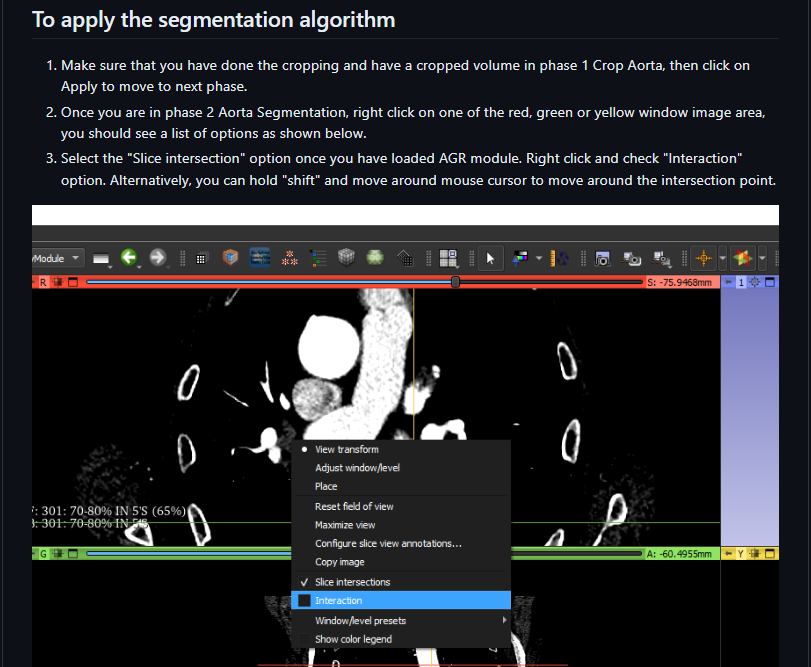
\includegraphics[width=0.9\textwidth]{figures/AC/GBA/User_manual.png}}
    \caption[AGR User Manual On GitHub README]{AGR User Manual On GitHub README}
    \label{fig_agr_git_um}
\end{figure}


\subsection{User Instruction Video}
Videos are an effective way to engage your audience and deliver information in a way that's easy to follow along and understand. A better instructional content is a YouTube Video where I make step-by-step instruction with voice over to instruct user. The Figure~\ref{fig_video} shows the playing video on YouTube. The video is not listed publicly on YouTube, but the users who have access to the GitHub repository or Design Document website can access this video by the \href{https://www.youtube.com/watch?v=1eK5k6bazNs}{URL link}.

\begin{figure}[H]
    \centering
    \fbox{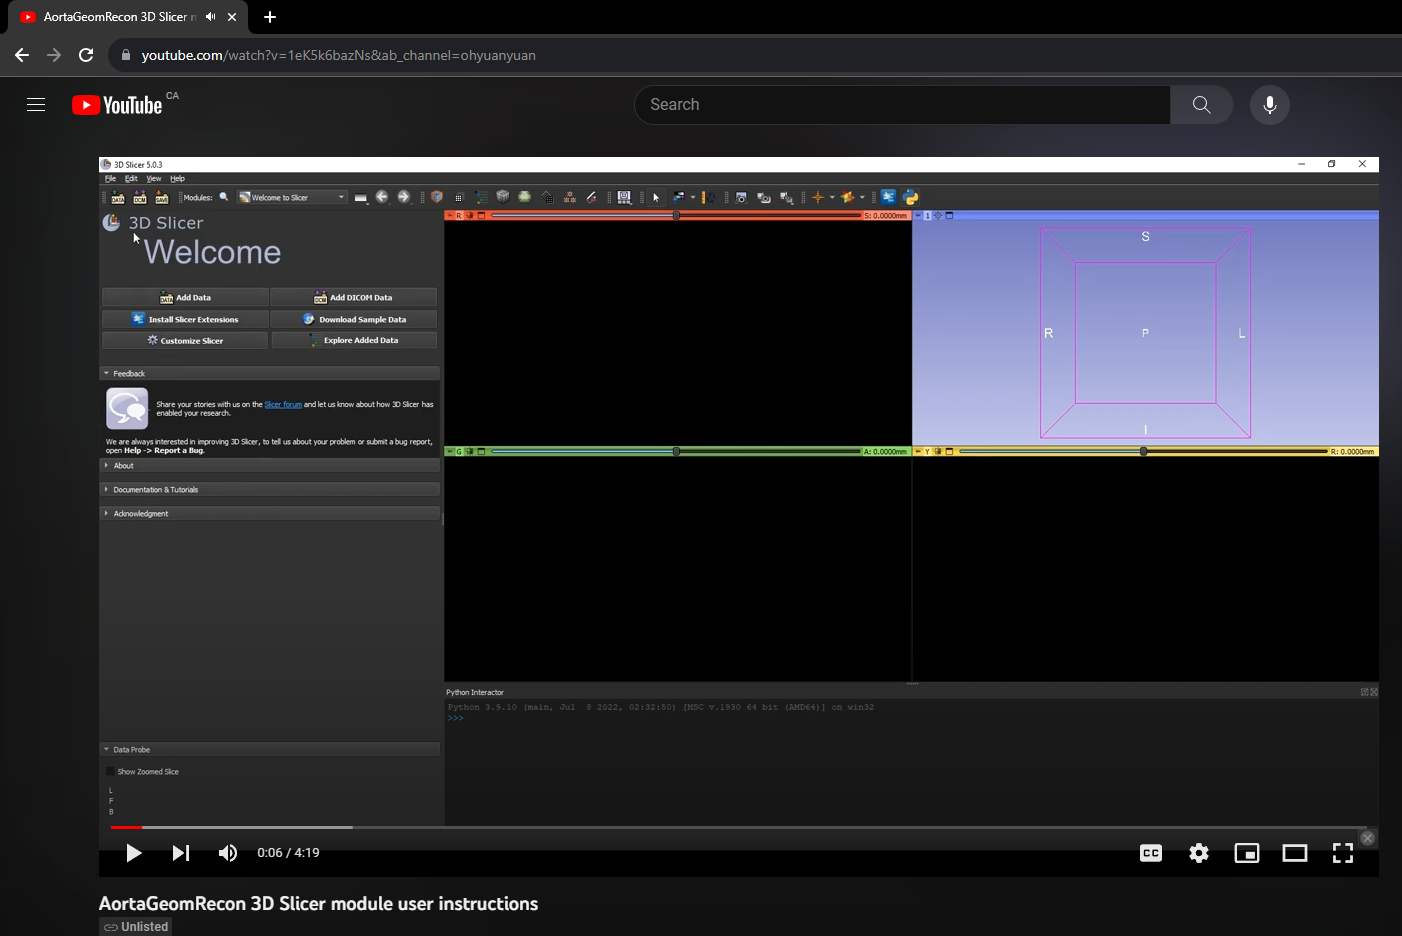
\includegraphics[width=0.8\textwidth]{figures/AC/GBA/User_instructions_video.png}}
    \caption[AGR User Instructions on YouTube]{AGR User Instructions on YouTube}
    \label{fig_video}
\end{figure}


\section{Assurance Case for Inputs Assumptions}

\begin{figure}[H]
    \centering
    \fbox{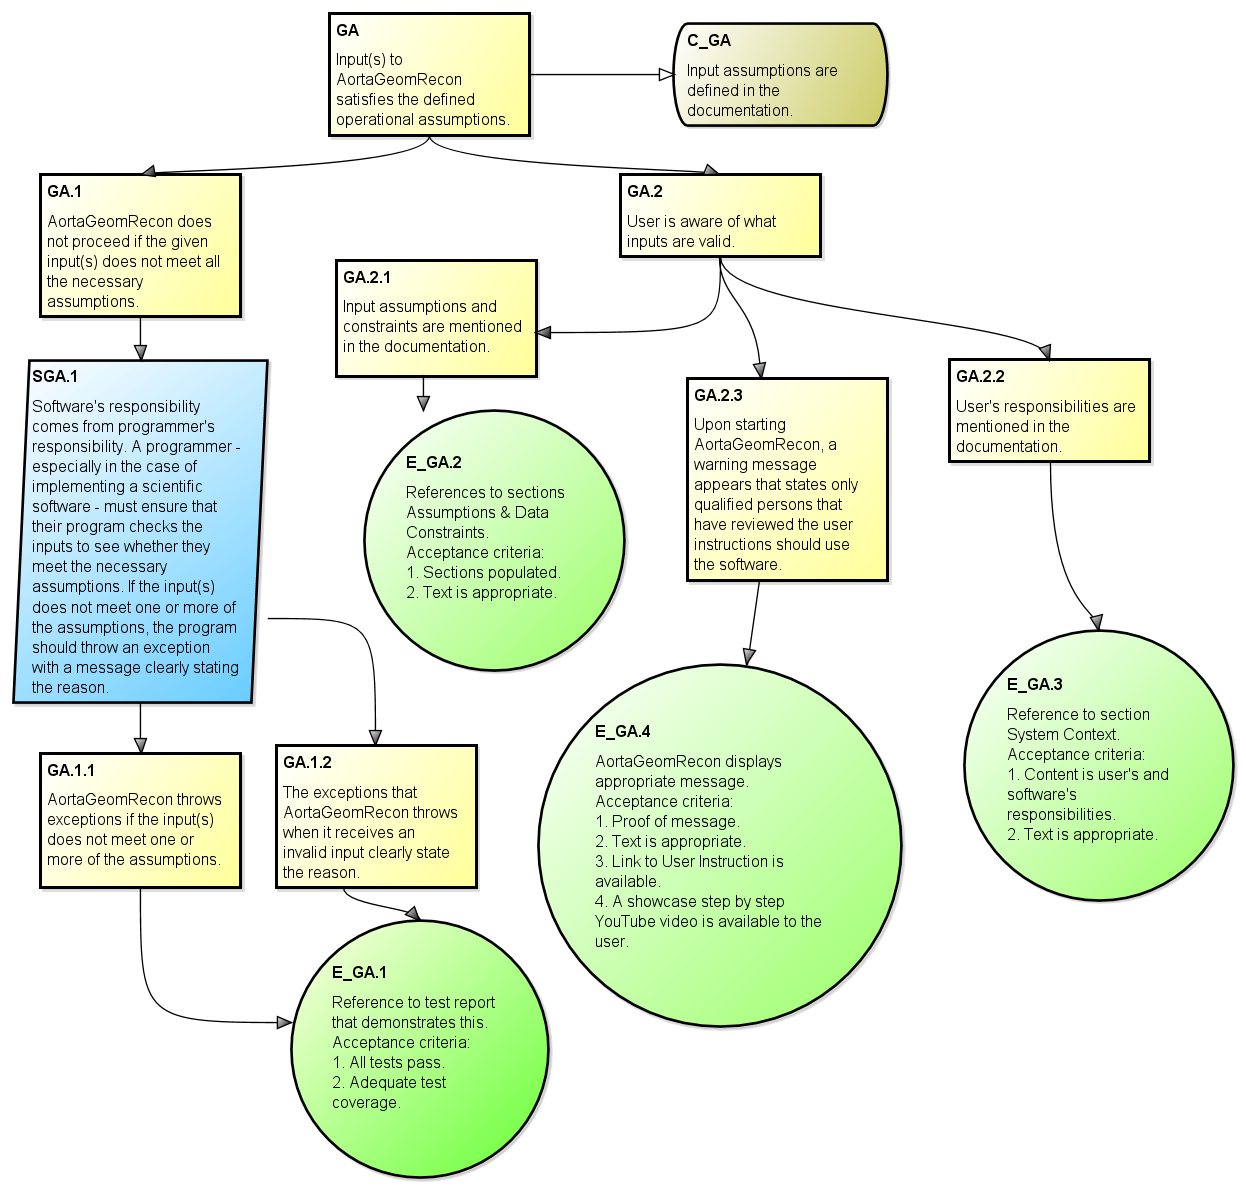
\includegraphics[width=\textwidth]{figures/AC/GA/GSN_GA.png}}
    \caption[AGR Assurance Case Inputs Assumptions]{AGR Assurance Case Inputs Assumptions}
    \label{fig_agr_ac_ga}
\end{figure}

The Figure~\ref{fig_agr_ac_ga} shows our last assurance case, GA. This statement requires the user know what inputs are valid, and only uses the valid inputs in the software. When the software gets unexpected inputs, it should not proceed to the next step, which could result in unexpected outputs.

\subsection{AortaGoemRecon's Control Sequence}

In the logic of the control sequence implemented as the 3D Slicer scripted module, the appropriate inputs must meet the necessary assumptions before proceed into the next step.
In phase one, a cropped volume with a name that includes the string ``cropped" must be present in the node storage, where a cropped volume created by Crop Volume module will automatically named with the string ``cropped" as part of the volume's name. Otherwise, the user cannot go to the next phase through normal operation. In phase two, the aorta seeds must be provided to continue to the segmentation. This implies that our evidence E\_GA.1 is satisfied.

\subsection{Warning Message}

As I initially planned, the references to sections Assumptions, Data Constraints, and System Context is available in the User Manual and User Instruction Video, where I showed the user how to import DICOM patient's data, and operate on the inputs' data till I get a segmentation result. This implies that the requirements of  the evidences E\_GA.2, E\_GA.3 and E\_GA.4 are met. A user who has read the User Manual and watched the instruction video should know what inputs are valid. Therefore, in the AGR module, I need to effectively guide the user to the User Manual, whether the user has used this software before or is a first time user.

\begin{figure}[H]
    \centering
    \fbox{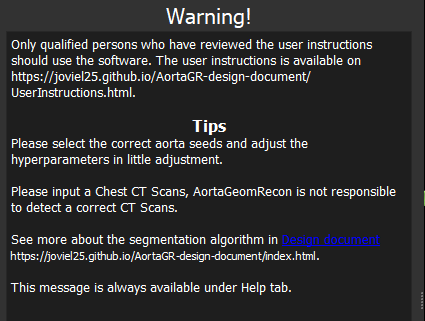
\includegraphics[width=0.6\textwidth]{figures/AC/GA/AGR_warning.png}}
    \caption[AGR Warning Message]{AGR Warning Message}
    \label{fig_agr_ac_wm}
\end{figure}

As mentioned in the section \ref{module_workflow}, when the user first starts 3D Slicer and click on the AGR module, this warning message appears, which is also referred as the appropriate message stated in E\_GA.4. The user must clicks on the Confirm button to continue to the next steps. With the warning message shown to the user, it is now the user's responsibility to use the valid inputs for AGR, which the program will deliver the correct outputs if the other operations are performed correctly. 

%Here is a sample equation (Equation~\ref{eq_lineslope}):
%
%\begin{equation} \label{eq_lineslope}
%	y = mx + b
%\end{equation}